\documentclass{beamer}
  \usepackage[utf8]{inputenc}
  \usetheme{Warsaw}
  \graphicspath{images/}
  \usepackage{amsmath}
  \usepackage{amssymb}
  \usepackage{verbatim}
  \usepackage{csquotes}
  \usepackage{graphicx}
  \usepackage{easyfig}
  % \usepackage[export]{adjustbox}
  \title{SEC313 : Développement d'applications sécurisées - CTF}
  \author{UFR des Sciences Versailles - M2 SeCReTS}
  \institute{AYOUB Pierre \& CAUMES Clément \& \\ DEBROUASSE Kevin \& Mehdi MTALSI-MERIMI}
  \date{110-broadcast-rsa-2 \\ 114-reversing-3 \\ 118-wpa-forensics}
  \begin{document}

  \begin{frame}
  \titlepage
  \end{frame}


	\section{110-broadcast-rsa-2}
	\begin{frame}
	\begin{block}{110-broadcast-rsa-2}
		\begin{itemize}
			\setbeamertemplate{itemize item}[circle]
			\item Introduction
			\item Description de la problématique
			\item Méthode générale de résolution
			\item Détails sur la résolution
			\item Ouverture
		\end{itemize}
	\end{block}

	\end{frame}

	\subsection{Introduction}

	\begin{frame}
	\begin{block}{Ce qu'on connaît}
		\begin{itemize}
			\setbeamertemplate{itemize item}[circle]
			\item Alice veut envoyer 1 même message à Bob, Charlie et Damien
			\item Bob, Charlie et Damien ont chacun une paire de clés asymétrique RSA et Alice connaît leurs clés publiques
			\item Alice chiffre le message avec un algorithme symétrique et chiffre la clé symétrique avec les clés publiques des 3 destinataires
		\end{itemize}
	\end{block}

	\begin{block}{Ce qu'on possède}
		\begin{itemize}
			\setbeamertemplate{itemize item}[circle]
			\item 1 fichier chiffré \textbf{ciphertext.bin}
			\item 3 fichiers chiffrés \textbf{enveloppe1.bin}, \textbf{enveloppe2.bin} et \textbf{enveloppe3.bin}
			\item 3 clés publiques \textbf{pubkey1.pem}, \textbf{pubkey2.pem} et \textbf{pubkey3.pem}
		\end{itemize}
	\end{block}

    \end{frame}

	\subsection{Description de la problématique}

	\begin{frame}
	\begin{block}{Ce que l'on cherche}
		\begin{itemize}
		\item Nous sommes Oscar et nous voulons connaître le contenu du message envoyé par Alice
		\end{itemize}
	\end{block}
	\begin{block}{Comment réussir l'attaque?}
		\begin{itemize}
		\item Trouver un moyen de calculer la clé symétrique en attaquant l'algorithme RSA (étape 1)
		\item Déchiffrer le message initial avec la clé symétrique qui vient d'être calculée (étape 2)
		\end{itemize}
	\end{block}
    \end{frame}

	\subsection{Méthode générale de résolution}
    \begin{frame}
	\begin{block}{Etape 1.1}
		\begin{itemize}
		\item Interpréter les 3 clés publiques utilisés pour chiffrer la clé symétrique choisi par Alice. Ces clés sont écrites sous le format \textbf{PEM} et sont codés en Base64. On obtiendra \textbf{n} et \textbf{e}.
		\end{itemize}
	\end{block}
	\begin{exampleblock}{Application au problème}
		Les trois destinataires possède le même \textbf{n}!
	\end{exampleblock}
	\end{frame}
	\begin{frame}
	\begin{block}{Etape 1.2}
		\begin{itemize}
			\item Interpréter les 3 enveloppes qui sont le résultat du chiffrement asymétrique avec les 3 clés publiques des destinataires. On doit donc traduire les octets en entier.
		\end{itemize}
	\end{block}

	\begin{exampleblock}{Application au problème}
		Le chiffrement asymétrique RSA correspond à : $c \equiv m^e [n]$ \\
		On obtient donc mathématiquement :
		\begin{itemize}
			\item $c_1 \equiv m^3$ $mod$ $n_1 \Leftrightarrow m^3 \equiv c_1$ $mod$ $n_1$
			\item $c_2 \equiv m^3$ $mod$ $n_2\Leftrightarrow m^3 \equiv c_2$ $mod$ $n_2$
			\item $c_3 \equiv m^3$ $mod$ $n_3\Leftrightarrow m^3 \equiv c_3$ $mod$ $n_3$
		\end{itemize}
		(avec $c_i$ l'enveloppe $i$, $e=3$ l'exposant publique des destinataires utilisé par Alice et $n_i$ le module du destinataire $i$).
	\end{exampleblock}
	\end{frame}
	\begin{frame}
		\begin{block}{Etape 1.3}
			\begin{itemize}
				\item Par l'application du théorème des restes chinois, on trouve $m^3$.
				\item Sachant que les exposants publiques choisis par les destinataires sont très petits (ici $3$), on peut facilement calculer la racine cubique de $m^3$ et ainsi trouver $m$.
				\item $m$ (qui est en réalité un nombre) est maintenant traduit en octets car c'est un message texte.
			\end{itemize}
		\end{block}
		\begin{exampleblock}{Application au problème}
			On obtient donc $m$ :

			\tiny{Are we there yet?\\
				--------------     Almost there!      -----------------\\
				filename: ciphertext.bin\\
				cipher: camellia-256-ofb\\
				key: EAEC5BA147E9C823C64CC9914D13779979D255E5CF615EA89789C564768FCB3A\\
				iv: 9E20C0E3D433BFF7F37ECC7B74091EF8\\}
		\end{exampleblock}
    \end{frame}

	\begin{frame}
		\begin{block}{Etape 2}
			Les enveloppes envoyées par Alice contenait le nom du chiffrement (Camellia), le mode opératoire (OFB), la clé 256 bits et le vecteur d'initialisation. \newline
			On peut donc déchiffrer \textbf{ciphertext.bin} qui est en réalité un fichier HTML contenant le flag.
		\end{block}
		\begin{center}
		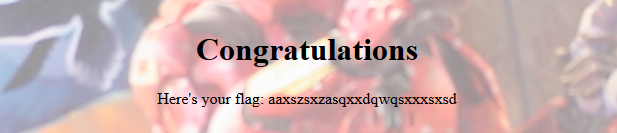
\includegraphics[scale=0.6]{./pictures/110-broadcast-rsa-2.PNG}
		\end{center}
	\end{frame}

	\subsection{Détails sur la résolution}

	\begin{frame}{Hastad's broadcast attack}
		L'attaque réalisée est l'\textbf{attaque broadcast de Hastad}. Elle est rendue possible par le fait que Alice a envoyé le même message à 3 destinataires différents et qui possèdent un exposant de chiffrement petit (ici $3$). Il met en jeu le \textbf{théorème des restes chinois} et le calcul d'une \textbf{racine cubique}.
	\end{frame}

	\begin{frame}{Théorème des restes chinois}
		\begin{block}{Théorème}
				L'inconnu est $x$ et nous avons les équations suivantes :
				\begin{itemize}
				\item $x \equiv a_1$ $mod$ $m_1$
				\item $x \equiv a_2$ $mod$ $m_2$
				\item $x \equiv a_3$ $mod$ $m_3$
				Si $m_i$ et $m_j$ premiers deux à deux alors on peut calculer : \newline
				\color{red}$x \equiv \sum \limits_{i=0}^{n}a_i \times M_i \times N_i$ $mod$ $M$ \color{black}

				avec $M_i=M / m_{i}$ et $N_i = Mi^{-1}$ $mod$ $m_i$
			\end{itemize}
		\end{block}
	\end{frame}

	\begin{frame}{Théorème des restes chinois}
	\begin{alertblock}{Démonstration pour comprendre l'attaque - Partie 1}
		\begin{itemize}
		\item Pour chaque $i$ les entiers $m_i$ et $M_i=M/m_i$ sont premiers entre eux.
		\item Avec l'algorithme d'Euclide étendu, on a deux coefficients de Bézout $u_i$ et $N_i$ tels que :
		$u_i\times m_i + N_i\times M_i = 1$ \newline $\Leftrightarrow N_i \times M_i = 1 - u_i \times m_i$ \newline $\Leftrightarrow N_i \times M_i \equiv 1$ $mod$ $m_i$ $et$ $N_i \times M_i \equiv 0$ $mod$ $m_j$
		\item Or, on a : $x \equiv a_i \times N_i \times M_i$ $mod$ $m_i$ \newline $\Leftrightarrow x \equiv a_i \times (1 - u_i \times m_i)$ $mod$ $m_i$ \newline
		$\Leftrightarrow x \equiv a_i \times 1$ $mod$ $m_i$ \newline
		$\Leftrightarrow x \equiv a_i$ $mod$ $m_i$
		\end{itemize}
	\end{alertblock}
	\end{frame}

	\begin{frame}{Théorème des restes chinois}
	\begin{alertblock}{Démonstration pour comprendre l'attaque - Partie 2}
	\begin{itemize}
		\item Supposons que $x'$ est également une solution.
		Donc, on a : \newline $x \equiv a_i \equiv x'$ $mod$ $m_i$
		$\Leftrightarrow m_i | (x-x')$
		\item Comme $m_i$ et $m_j$ sont premiers entre eux, alors $x \equiv x'$ $mod$ $M$
		\item Donc : $x \equiv \sum \limits_{i=0}^{n}a_i \times M_i \times N_i$ $mod$ $M$
		\item On pouvait donc bien utiliser ce théorème pour résoudre notre problème initial et trouver $m^3$
	\end{itemize}
	\end{alertblock}
	\end{frame}

	\subsection{Ouverture}

	\begin{frame}
	\begin{block}{Comment éviter cette attaque?}
		\begin{itemize}
			\item Arrêter d'envoyer le même message à plusieurs différentes? Difficile à mettre en place
			\item Insérer de l'aléatoire pour que chaque destinataire reçoive un message différent : PKCS\#1 v1.5
		\end{itemize}
	\end{block}
	\begin{exampleblock}{PKCS\#1 v1.5}
	$C=(\mu(M))^e$ $mod$ $n$ avec
	$\mu(M)=\O\O\O2||r||\O\O||M$ \newline dont $r$ est une valeur aléatoire d'au moins 8 octets
	\end{exampleblock}
	\end{frame}

	\section{114-reversing-3}

	\begin{frame}
	\begin{block}{114-reversing-3}
		\begin{itemize}
			\setbeamertemplate{itemize item}[circle]
			\item Introduction
			\item Description de la problématique
			\item Méthode générale de résolution
			\item Détails sur la résolution
			\item Ouverture
		\end{itemize}
	\end{block}

	\end{frame}

	\subsection{Introduction}

	\begin{frame}

	\begin{block}{Ce qu'on possède}
		\begin{itemize}
			\setbeamertemplate{itemize item}[circle]
			\item 1 fichier exécutable \textbf{encoreunflag}
		\end{itemize}
	\end{block}

	\begin{block}{Ce qu'on connaît}
	\begin{itemize}
		\setbeamertemplate{itemize item}[circle]
		\item Aucun indice de fourni, on ne sait même pas si il y a éventuellement des paramètres. En exécutant le programme, on nous suggère de mettre en argument un mot de passe que l'on ne connaît pas (encore).
	\end{itemize}
	\end{block}

	\end{frame}

	\subsection{Description de la problématique}

	\begin{frame}
	\begin{block}{Ce que l'on cherche}
		\begin{itemize}
			\item Nous voulons connaître le mot de passe pour s'authentifier
		\end{itemize}
	\end{block}
	\begin{block}{Comment réussir l'attaque?}
		\begin{itemize}
			\item Faire du reverse engineering afin de trouver quel mot de passe est valide
		\end{itemize}
	\end{block}
	\end{frame}

	\subsection{Méthode générale de résolution}
	\begin{frame}
	\begin{block}{Etape 1.1}
		\begin{itemize}
			\item Le premier réflexe est d'ouvrir le programme avec le désassembleur \textbf{IDA}.
			\item Le premier bloc d'exécution se termine par une condition sur le nombre d'arguments en ligne de commandes
		\end{itemize}
	\end{block}
	\begin{exampleblock}{Condition sur le nombre d'arguments}
		\begin{center}
			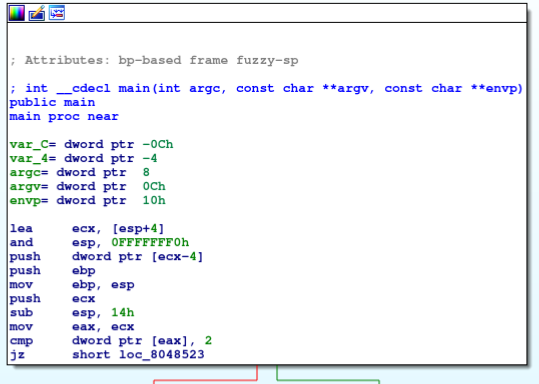
\includegraphics[scale=0.4]{./pictures/114-reversing-3-1.PNG}
		\end{center}
	\end{exampleblock}
	\end{frame}

	\begin{frame}
	\begin{block}{Etape 1.2}
		\begin{itemize}
			\item Si on ne met pas 2 arguments, le programme se terminera (donc si il n'y a pas le mot de passe en argument de la commande)
		\end{itemize}
	\end{block}
	\begin{exampleblock}{Si le nombre d'arguments est incorrect}
		\begin{center}
			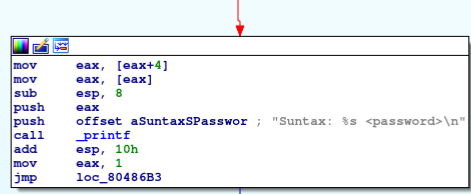
\includegraphics[scale=0.45]{./pictures/114-reversing-3-2.PNG}
		\end{center}
	\end{exampleblock}
	\end{frame}

	\begin{frame}
		\begin{block}{Etape 1.3}
		\begin{itemize}
		\item Sinon, on continue la batterie de tests
		\item Ce nouveau bloc d'exécution va appeler la fonction \textbf{strlen} et tester si la taille du mot de passe fait \textbf{0x14} soit \textbf{20 octets} (donc 20 caractères ASCII)
		\end{itemize}
		\end{block}
		\begin{exampleblock}{Vérification de la taille du mot de passe}
		\begin{center}
			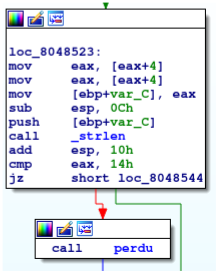
\includegraphics[scale=0.45]{./pictures/114-reversing-3-3.PNG}
		\end{center}
		\end{exampleblock}
	\end{frame}

	\subsection{Détails sur la résolution}

	\begin{frame}{Coeur du programme}
		\begin{block}{Etape 3}
			\begin{itemize}
				\item Le programme réalise plusieurs tests conditionnels successifs qui se ressemble beaucoup
			\end{itemize}
		\end{block}
		\begin{exampleblock}{Tests successifs}
			\begin{center}
				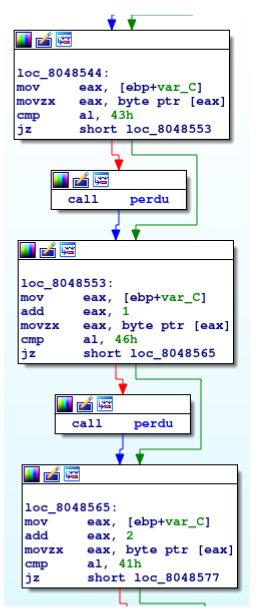
\includegraphics[scale=0.4]{./pictures/114-reversing-3-4.PNG}
			\end{center}
		\end{exampleblock}
	\end{frame}

	\begin{frame}
		\begin{block}{Compréhension de la série de tests}
			\begin{itemize}
				\item byte ptr[n] permet de récupérer l’octet à la position n
				\item chaque bloc compare donc chaque octet du mot de passe à la position n avec un octet particulier
				\item récupérons ces différents octets écrits en hexadécimal
			\end{itemize}
		\end{block}
		\begin{exampleblock}{Récupération des octets comparés du programme}
			\begin{itemize}
			\item 43 46 41 54 4c 59 6f 6a 74 72 48 75 4d 52 5a 49 4a 6b 71 78
			\end{itemize}
			\begin{center}
			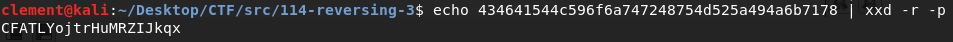
\includegraphics[scale=0.4]{./pictures/114-reversing-3-6.PNG}
			\end{center}
			\begin{itemize}
				\item Solution :
			\end{itemize}
			\begin{center}
				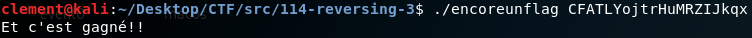
\includegraphics[scale=0.4]{./pictures/114-reversing-3-5.PNG}
			\end{center}
		\end{exampleblock}
	\end{frame}

	\subsection{Ouverture}

	\begin{frame}
	\begin{block}{Comment éviter cette attaque?}
		\begin{itemize}
		\item Utiliser une fonction de hachage robuste et un salt
		\item Le programme comparera le hash du salt concaténé au mot de passe de l'utilisateur pour vérifier l'authentification.
		\end{itemize}
	\end{block}
	\end{frame}

	\section{118-wpa-forensics}

	\begin{frame}
	\begin{block}{118-wpa-forensics}
		\begin{itemize}
		\setbeamertemplate{itemize item}[circle]
		\item Introduction
		\item Description de la problématique
		\item Méthode générale de résolution
		\item Détails sur la résolution
		\item Ouverture
		\end{itemize}
	\end{block}

	\end{frame}

	\subsection{Introduction}

	\begin{frame}

	\begin{block}{Ce qu'on possède}
		\begin{itemize}
			\setbeamertemplate{itemize item}[circle]
			\item 1 fichier de captures de trafic réseau interceptés sur le lieu à attaquer
		\end{itemize}
	\end{block}

	\begin{block}{Ce qu'on connaît}
		\begin{itemize}
			\setbeamertemplate{itemize item}[circle]
			\item Le lieu à attaquer utilise un réseau Wifi WPA-PSK
			\item Le mot de passe Wifi est un mot anglais de 10 lettres (majuscules) suivies de 2 chiffres
		\end{itemize}
	\end{block}

	\end{frame}

	\subsection{Description de la problématique}

	\begin{frame}
	\begin{block}{Ce que l'on cherche}
		\begin{itemize}
			\item Nous voulons connaître le mot de passe du serveur web utilisé par notre victime
		\end{itemize}
	\end{block}
	\begin{block}{Comment réussir l'attaque?}
		\begin{itemize}
			\item Le contenu du trafic est protégé par du chiffrement dû à l'utilisation du WPA-PSK. Il faut donc réussir à déchiffrer le trafic réseau.
			\item Il faut ensuite analyser le trafic réseau pour trouver le mot de passe utiliser pour s'authentifier auprès du serveur web.
		\end{itemize}
	\end{block}
	\end{frame}

	\subsection{Méthode générale de résolution}

	\begin{frame}
	\begin{block}{Description générale de WPA-PSK}
		\begin{itemize}
			\item Il s'appuie sur un mécanisme d'authentification EAP (sous forme de challenge-réponse)
			\item Il utilise le protocole EAPoL (Extensible Authentication Protocol over LAN)
		\end{itemize}
	\end{block}

	\begin{block}{Préliminaires}
		\begin{itemize}
			\item Le fournisseur d'accès et le client connaissent le SSID (l'identifiant du fournisseur d'accès) et la PSK (le mot de passe "Wifi").
			\item Le fournisseur d'accès et le client déduisent la PMK (clé maître) qu'ils stockent chacun de leurs côtés.
			\item $PMK = PBKDF2(HMAC-SHA1, PSK, SSID, 4096, 256)$
			C'est une fonction de hachage HMAC-SHA1 qui fera 4096 itérations (pour rendre plus lent l'attaque brute-force)
		\end{itemize}
	\end{block}
	\end{frame}

	\begin{frame}{HandShake en 4 temps}
		\begin{center}
			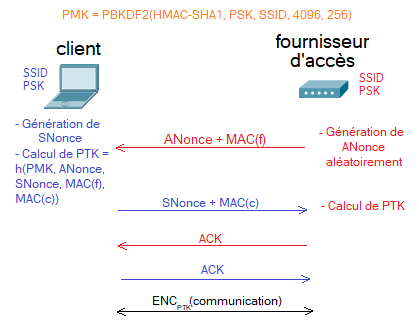
\includegraphics[scale=0.7]{./pictures/118-wpa-forensics-schema.PNG}
		\end{center}
	\end{frame}

	\begin{frame}
	\begin{block}{Description générale de l'attaque}
		\begin{itemize}
			\item Ecoute du trafic réseau et attente d'une nouvelle connexion
			\item Capture du HandShake en 4 temps
			\item Récupération de $ANonce$, $SNonce$ et des adresses MAC du client et du fournisseur d'accès
			\item Attaque par dictionnaire pour trouver un PSK qui puisse correspondre pour déchiffrer leurs communications (avec la PTK associée)
			\item $\color{red}PMK\color{black} = h(\color{red}PSK\color{black}, \color{green}SSID\color{black})$ \newline
			$\color{red}PTK\color{black} = h'(\color{red}PMK\color{black}, \color{green}ANonce\color{black}, \color{green}SNonce\color{black}, \color{green}MAC_C\color{black}, \color{green}MAC_F\color{black})$
		\end{itemize}
	\end{block}
	\end{frame}

	\subsection{Détails sur la résolution}

	\begin{frame}
	\begin{block}{Etape 1}
		\begin{itemize}
			\item L'indice indique que la PSK est un mot anglais de 10 lettres suivi de deux chiffres
			\item En cherchant sur Internet, \href{www.bestwordlist.com/10letterwords.htm} propose une liste de mots anglais en majuscules (dispersées sur 79 pages web)
			\item Ecriture d'un script qui va télécharger le contenu des 79 pages et parser le résultat
			\item Ecriture des mots concaténés à 2 chiffres (de $00$ à $99$)
			\item Récupération de notre fichier \textbf{wordlist.txt}
		\end{itemize}
	\end{block}
	\end{frame}

	\begin{frame}
	\begin{block}{Etape 2}
		\begin{itemize}
			\item Utilisation de l'outil \textbf{aircrack-ng} : \newline $aircrack$-$ng$ -$w$ $wordlist.txt$ $psk$-$01$.$cap$
			\item Récupération de la \textbf{PSK}
		\end{itemize}
	\end{block}
	\begin{exampleblock}{Utilisation de aircrack-ng}
		\begin{center}
				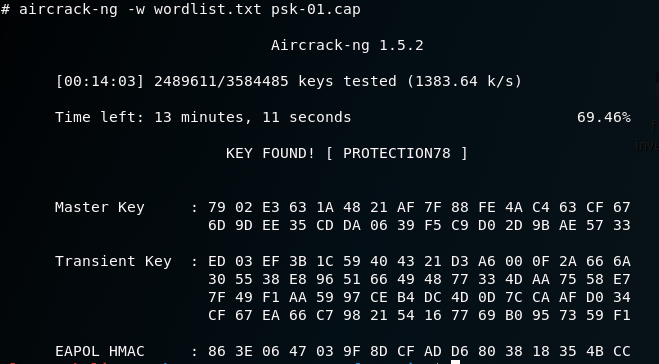
\includegraphics[scale=0.4]{./pictures/118-wpa-forensics-aircrackng.PNG}
		\end{center}
	\end{exampleblock}
	\end{frame}

	\begin{frame}
	\begin{block}{Etape 3}
		Edition de la PSK sur Wireshark :
		\begin{itemize}
			\item Déduction de la PMK puis de la PTK
			\item Traduction du trafic
		\end{itemize}
	\end{block}
	\begin{exampleblock}{Utilisation sur Wireshark}

			\begin{itemize}
				\item Ajout de la PSK et du SSID
			\end{itemize}
			\begin{center}
				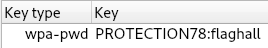
\includegraphics[scale=0.6]{./pictures/118-wpa-forensics-wireshark-pwd.png}
			\end{center}
			\begin{itemize}
				\item Déchiffrement automatique des communications
			\end{itemize}
			\begin{center}
				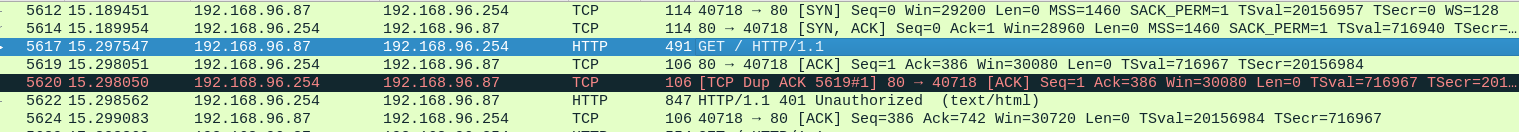
\includegraphics[scale=0.25]{./pictures/118-wpa-forensics-wireshark-http.png}
			\end{center}

	\end{exampleblock}
	\end{frame}

	\begin{frame}{Solution}
		\begin{center}
			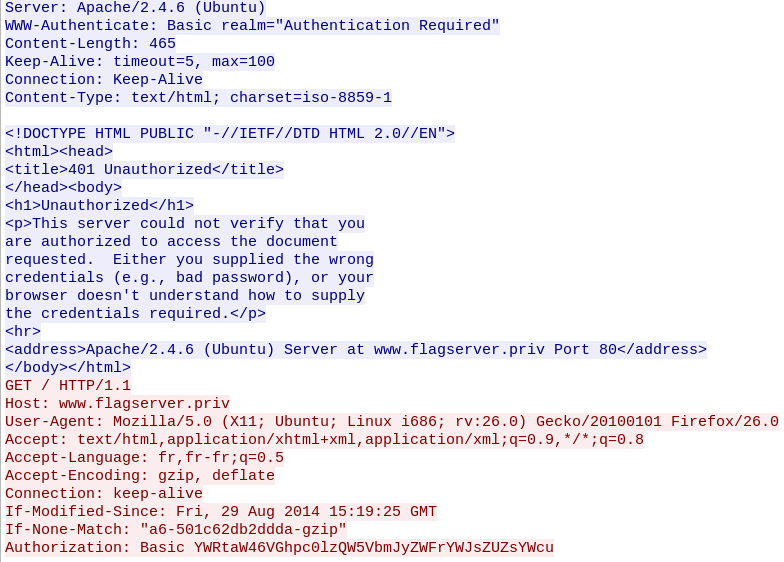
\includegraphics[scale=0.4]{./pictures/118-wpa-forensics-wireshark-follow.png}
		\end{center}
		\begin{center}
			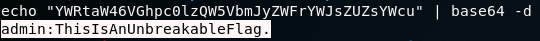
\includegraphics[scale=0.5]{./pictures/118-wpa-forensics-flag.png}
		\end{center}
	\end{frame}

	\subsection{Ouverture}

	\begin{frame}
	\begin{block}{Comment éviter cette attaque?}
		Paramétrer une clé PSK robuste :
		\begin{itemize}
			\item au minimum 16 caractères
			\item mélangeant minuscules, majuscules, chiffres et caractères spéciaux
			\item à générer de manière (pseudo) aléatoire
		\end{itemize}
	\end{block}
	\begin{alertblock}{Dernier détail!}
		Il faut changer le mot de passe par défaut (même s'il semble robuste) car ces mots de passe par défaut suivent la plupart du temps un pattern connu par les attaquants
	\end{alertblock}
	\begin{block}{Ouverture sur WPA3}
		Lorsque WPA3 sera disponible, plutôt se tourner vers ce dernier car il utilise un autre protocole d'établissement de clé (SAE).
	\end{block}
	\end{frame}

	\section{122-nfs-and-remote-attack}

        \begin{frame}
            \begin{block}{122-nfs-and-remote-attack}
                \begin{itemize}
                        \setbeamertemplate{itemize item}[circle]
                    \item Introduction
                    \item Description de la problématique
                    \item Méthode générale de résolution
                    \item Détails sur la résolution
                    \item Ouverture
                \end{itemize}
            \end{block}
        \end{frame}

	\subsection{Introduction}

        \begin{frame}[fragile]
            \begin{block}{Ce qu'on possède}
                \begin{itemize}
                        \setbeamertemplate{itemize item}[circle]
                    \item Deux disques durs de machines virtuelles.
                \end{itemize}
            \end{block}
            \begin{block}{Ce qu'on connaît}
                \begin{itemize}
                        \setbeamertemplate{itemize item}[circle]
                    \item Accès au disque interdit autrement que par un utilisateur légitime.
                    \item Deux accès possibles : console et réseau.
                    \item Mode live, DHCP, services réseaux.
                    \item Export NFS de \verb+/home/bob+ (droit \verb+rw+ et pas de \enquote{root squashing}).
                    \item Utilisateur \verb+tc+ peut utiliser \verb+sudo+ sans mot de passe.
                \end{itemize}
            \end{block}
        \end{frame}

        \subsection{Description de la problématique}

        \begin{frame}[fragile]
            \begin{block}{Ce que l'on cherche}
                \begin{itemize}
                    \item Accéder au flag contenu dans \verb+/root/flag+.
                \end{itemize}
            \end{block}
            \begin{block}{Comment réussir l'attaque ?}
                \begin{itemize}
                    \item Accéder au compte d'un utilisateur (local et/ou réseau).
                    \item Élevation de privilège pour accéder au flag.
                \end{itemize}
            \end{block}
        \end{frame}

        \subsection{Méthode générale de résolution}

        \begin{frame}[t]
            \begin{block}{UNIX}
                \begin{itemize}
                    \item Identification des utilisateurs/groupes : UID et GID.
                    \item Permission SUID.
                \end{itemize}
            \end{block}
            \begin{block}{NFS}
                \begin{itemize}
                    \item Partage de fichiers via le système de montage (1984).
                    \item Filtrage par IP.
                    \item Droits UNIX.
                \end{itemize}
            \end{block}
            \begin{block}{SSH}
                \begin{itemize}
                    \item Authentification : mot de passe vs. clés RSA.
                \end{itemize}
            \end{block}
        \end{frame}

	\subsection{Détails sur la résolution}

        \begin{frame}[fragile]
            \begin{block}{Etape 1 -- Découverte}
                \begin{itemize}
                    \item \verb+nmap+ : on découvre l'IP, puis deux services : SSH et NFS (alternative : console).
                    \item \verb+showmount+ : utilitaire pour découvrir les exports NFS.
                \end{itemize}
            \end{block}
            \begin{exampleblock}{Illustration}
                \begin{center}
                    \Figure[max size={\textwidth}{.5\textheight}]{./pictures/nfs-1.png}
                \end{center}
            \end{exampleblock}
        \end{frame}

        \begin{frame}[fragile]
            \begin{block}{Étape 2 -- Usurpation de bob en local}
                \begin{itemize}
                    \item Montage de l'export NFS.
                    \item Récupération de l'UID de \verb+bob+.
                    \item Usurpation de \verb+bob+ en local.
                \end{itemize}
            \end{block}
            \begin{exampleblock}{Illustration}
                \begin{center}
                    \Figure[max size={\textwidth}{.5\textheight}]{./pictures/nfs-2.png}
                \end{center}
            \end{exampleblock}
        \end{frame}

        \begin{frame}[fragile]
            \begin{block}{Étape 3 -- Exploitation d'un accès SSH à bob}
                \begin{itemize}
                    \item Création d'une paire de clé RSA pour SSH.
                    \item Logging en tant que bob en local.
                    \item Ajout de la clé publique de l'utilisateur local (pierre).
                \end{itemize}
            \end{block}
            \begin{exampleblock}{Illustration}
                \begin{center}
                    \Figure[max size={\textwidth}{.5\textheight}]{./pictures/nfs-3.png}
                \end{center}
            \end{exampleblock}
        \end{frame}

        \begin{frame}[fragile]
            \begin{block}{Étape 4 -- Préparation à l'usurpation de tc}
                \begin{itemize}
                    \item Autorisation de tc à écrire dans \verb+/home/bob+.
                    \item Copie d'un shell dans le \verb+home+ de \verb+bob+.
                \end{itemize}
            \end{block}
            \begin{exampleblock}{Illustration}
                \begin{center}
                    \Figure[max size={\textwidth}{.5\textheight}]{./pictures/nfs-4.png}
                \end{center}
            \end{exampleblock}
        \end{frame}
        
        \begin{frame}[fragile]
            \begin{block}{Étape 5 -- Usurpation de tc en local}
                \begin{itemize}
                    \item Récupération de l'UID de \verb+tc+ en cherchant des
                        fichiers lui appartenant après la connexion SSH (caché).
                    \item Création d'un utilisateur avec l'UID adapté.
                \end{itemize}
            \end{block}
            \begin{exampleblock}{Illustration}
                \begin{center}
                    \Figure[max size={\textwidth}{.5\textheight}]{./pictures/nfs-5.png}
                \end{center}
            \end{exampleblock}
        \end{frame}

        \begin{frame}[fragile]
            \begin{block}{Étape 6 -- Exploitation du bit SUID}
                \begin{itemize}
                    \item Copie du shell en local.
                    \item Changement de propriétaire pour \verb+tc+.
                    \item Log avec \verb+tc+ pour avoir le droit de déplacer le shell
                        dans le dossier de \verb+bob+ et de placer le bit SUID
                        (puisque le fichier lui appartient).
                \end{itemize}
            \end{block}
            \begin{exampleblock}{Illustration}
                \begin{center}
                    \Figure[max size={\textwidth}{.5\textheight}]{./pictures/nfs-6.png}
                \end{center}
            \end{exampleblock}
        \end{frame}
        
        \begin{frame}[fragile]
            \begin{block}{Étape 7 -- Profit}
                \begin{itemize}
                    \item \verb+bob+ lance le shell : il obtient les droits de
                        \verb+tc+.
                    \item \verb+tc+ fait partit du groupe \verb+staff+ au même titre que
                        \verb+root+ : il peut lire le flag.
                \end{itemize}
            \end{block}
            \begin{exampleblock}{Illustration}
                \begin{center}
                    \Figure[max size={\textwidth}{.5\textheight}]{./pictures/nfs-7.png}
                \end{center}
            \end{exampleblock}
        \end{frame}
        
	\subsection{Ouverture}
        \begin{frame}
            \begin{block}{Comment éviter cette attaque (dans ce scénario) ?}
                \begin{itemize}
                    \item Utilisation d'IP statiques contrôlées.
                    \item Partage de dossiers de stockage et non utilisateurs.
                    \item Gestion des utilisateurs sur un serveur central.
                \end{itemize}
            \end{block}
            \begin{block}{Comment éviter cette attaque (dans la réalité) ?}
                \begin{itemize}
                    \item Utilisation de Kerberos avec NFSv4.
                \end{itemize}
            \end{block}
        \end{frame}

    \end{document}
